\documentclass{article}
\usepackage[utf8]{inputenc}
\usepackage{graphicx}

\begin{document}

\begin{figure}%[tbhp]
\centering
 \begin{minipage}{.3\textwidth}
   \centering
   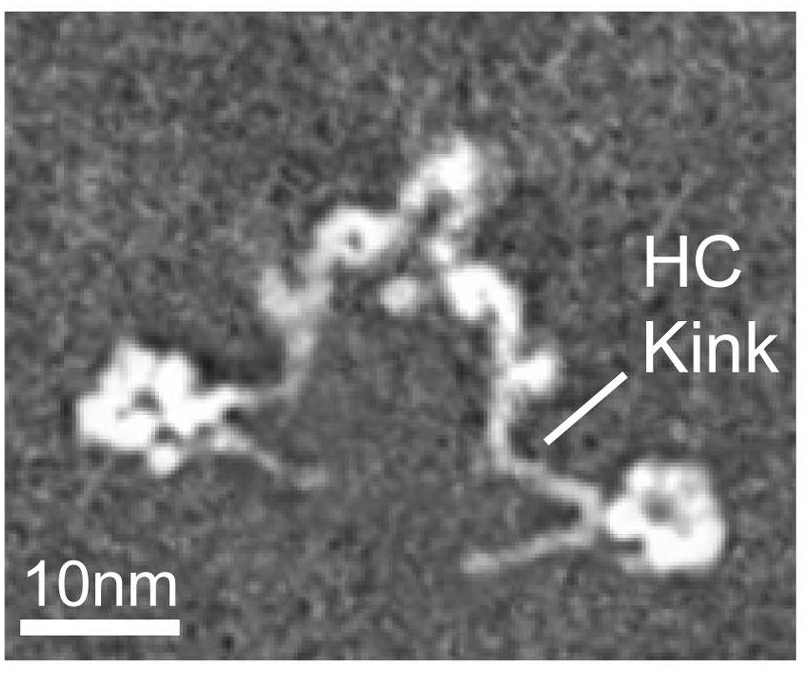
\includegraphics[width=\linewidth]{figures/schematic-1-cryoem}
   \caption{AAAAAAAA}
   \label{fig:modlengths}
 \end{minipage}%
 \begin{minipage}{.3\textwidth}
   \centering
   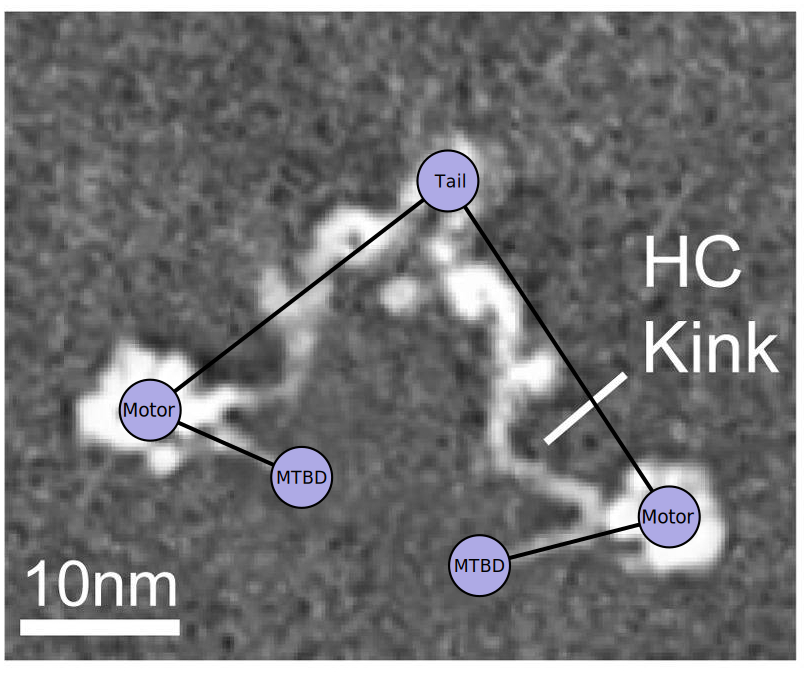
\includegraphics[width=\linewidth]{figures/schematic-1-superimposed}
   \caption{AAAAAAAA}
   \label{fig:modlengths}
 \end{minipage}%
 \begin{minipage}{.3\textwidth}
   \centering
   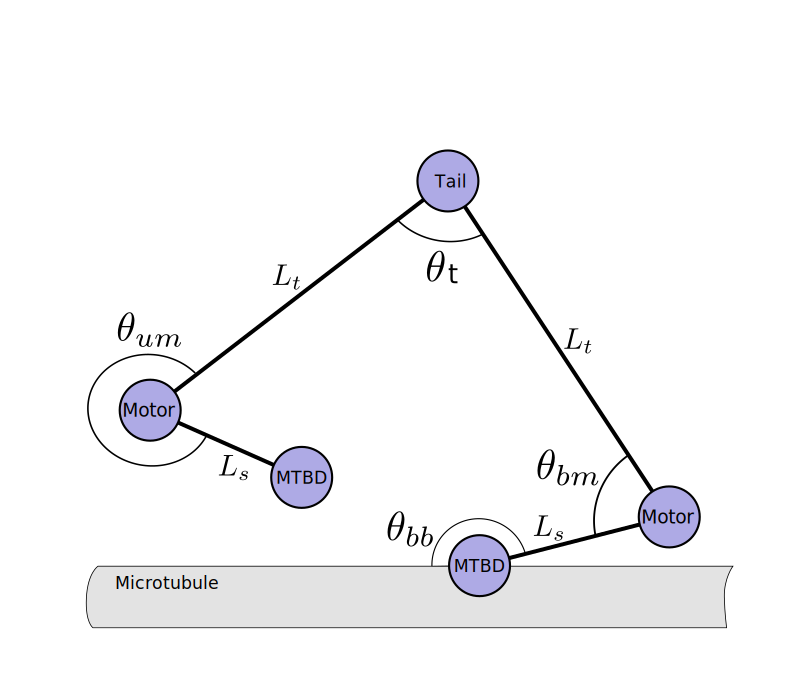
\includegraphics[width=\linewidth]{figures/schematic-1-model}
   \caption{AAAAAAAA}
   \label{fig:explengths}
 \end{minipage}
 \begin{minipage}{.5\textwidth}
   \centering
   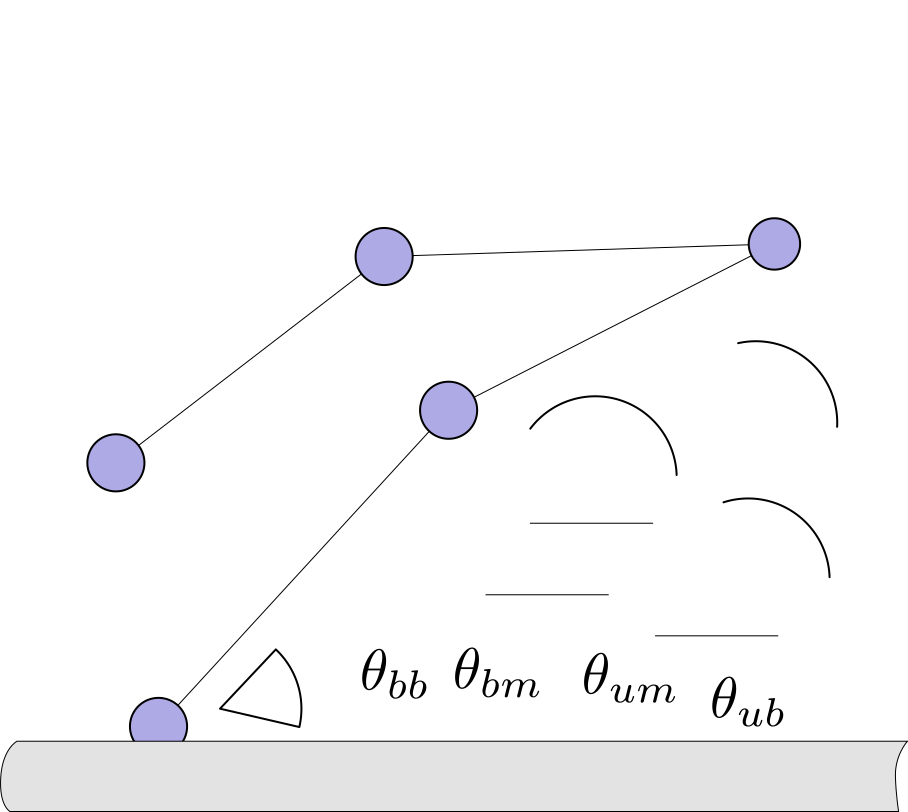
\includegraphics[width=\linewidth]{figures/ob_fig}
   \caption{AAAAAAAA}
   \label{fig:modangles}
 \end{minipage}%
 \begin{minipage}{.5\textwidth}
   \centering
   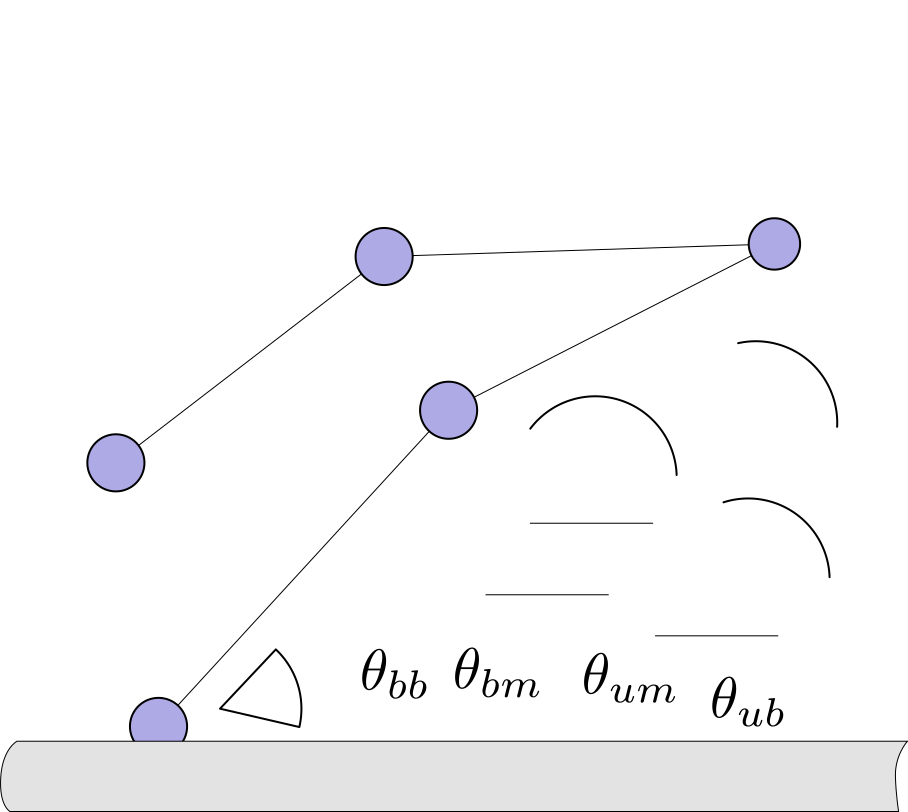
\includegraphics[width=\linewidth]{figures/ob_fig}
   \caption{AAAAAAAA}
   \label{fig:expangles}
 \end{minipage}
\caption{\textbf{Experimental values used to determine model parameters.}}
\label{fig:modelparams}
\end{figure}



\end{document}
